\documentclass[]{article}

% Imported Packages
%------------------------------------------------------------------------------
\usepackage{amssymb}
\usepackage{amstext}
\usepackage{amsthm}
\usepackage{amsmath}
\usepackage{enumerate}
\usepackage{fancyhdr}
\usepackage[margin=1in]{geometry}
\usepackage{graphicx}
\usepackage{extarrows}
\usepackage{setspace}
\usepackage{float}
%------------------------------------------------------------------------------

% Header and Footer
%------------------------------------------------------------------------------
\pagestyle{plain}  
\renewcommand\headrulewidth{0.4pt}                                      
\renewcommand\footrulewidth{0.4pt}   
\setlength{\parindent}{0em}
\setlength{\parskip}{1em}                              
%------------------------------------------------------------------------------

% Title Details
%------------------------------------------------------------------------------
\title{Deliverable \#3}
\author{   iSpaceship
        \\ Group 4, T02
        \\
		\\ Pedram Yazdinia, yazdinip
		\\ Will Conry, conrywm
		\\ Torja Istiaque, istiaqum
		\\ Akila Kavisinghe, kavisina
		\\ Xiangxin Kong, kongx9
}

\date{\today}                              
%------------------------------------------------------------------------------

% Document
%------------------------------------------------------------------------------
\begin{document}

\maketitle	

\section{Introduction}
\label{sec:introduction}
% Begin Section


\subsection{Purpose}
\label{sub:purpose}
% Begin SubSection
The purpose of this document is to define the flow of control between modules and classes, while also highlighting the implementation details for each class. This has been done through the use of various UML diagrams, including State Chart Diagrams, Sequence Diagrams, and Class Diagrams. Each diagram provides high level information about different pieces of the application. The intended audience for this document includes direct and indirect stakeholders, primarily Dr. Khedri, Andrew Le Clair, and the testing team. 
% End SubSection

\subsection{System Description}
\label{sub:system_description}
% Begin SubSection
 “iSpaceship” is a Rogue-like, turn-based, spaceship battle simulator, video game. The software product will provide the user with an engaging gaming experience where they can build their own spaceship and battle other spaceships. The software product will be used for the enjoyment of the user and provide them with a sense of self-accomplishment. The objective is for users to have fun and feel rewarded when they put in the time and dedication to progress in the game. The application should hold interest of users over a long period of time.

% End SubSection

\subsection{Overview}
\label{sub:overview}
% Begin SubSection
This document is divided into four sections, including the above Introduction section. In section 2, the state charts are given. The state diagrams show the program at different states and the properties of the attached transitions which include the event, guard (the condition), and the action. In section 3, the sequence diagrams are described. The diagrams in this section describe the communication between different classes, each diagram is derived from a use case. Finally in section 4, a detailed class diagram of the entire project is provided. This section outlines the implementation details for each class which includes the attributes, public and private methods, as well as the relation between the classes.

% End SubSection

% End Section

\section{State Charts for Controller Classes}
\label{sec:state_charts_for_controller_classes}
% Begin Section
\begin{figure}[H]
    \centering
    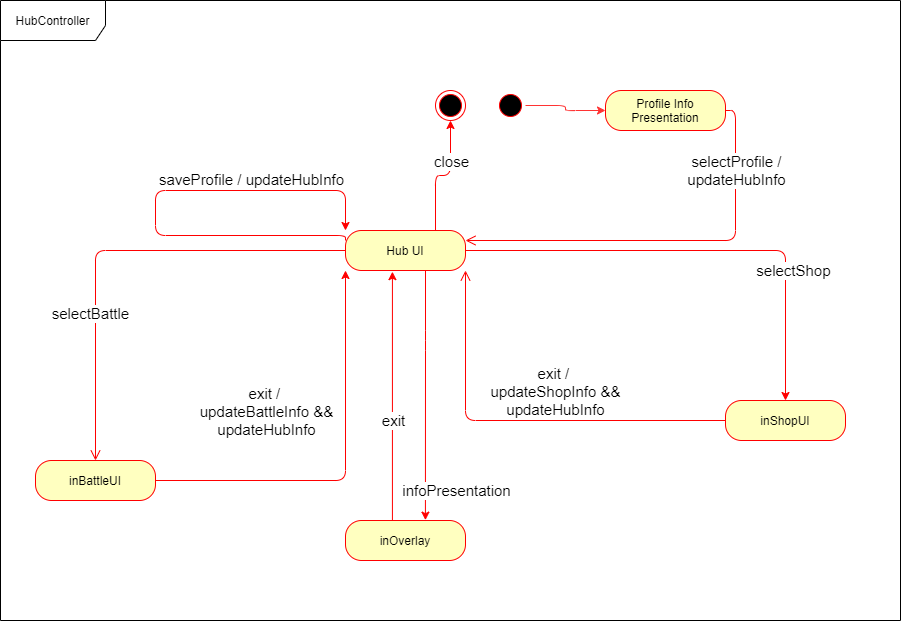
\includegraphics[width=\textwidth]{HubController.png}
    \caption{State Diagram for Hub Controller Class.}
    \label{fig:ca}
\end{figure}

\begin{figure}[H]
    \centering
    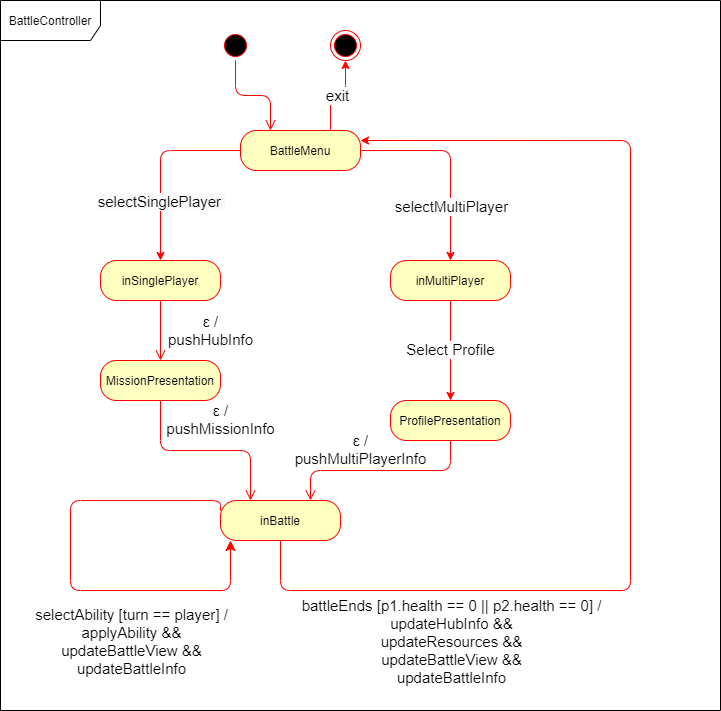
\includegraphics[width=\textwidth]{BattleController.png}
    \caption{State Diagram for Battle Controller Class.}
    \label{fig:ca}
\end{figure}

\begin{figure}[H]
    \centering
    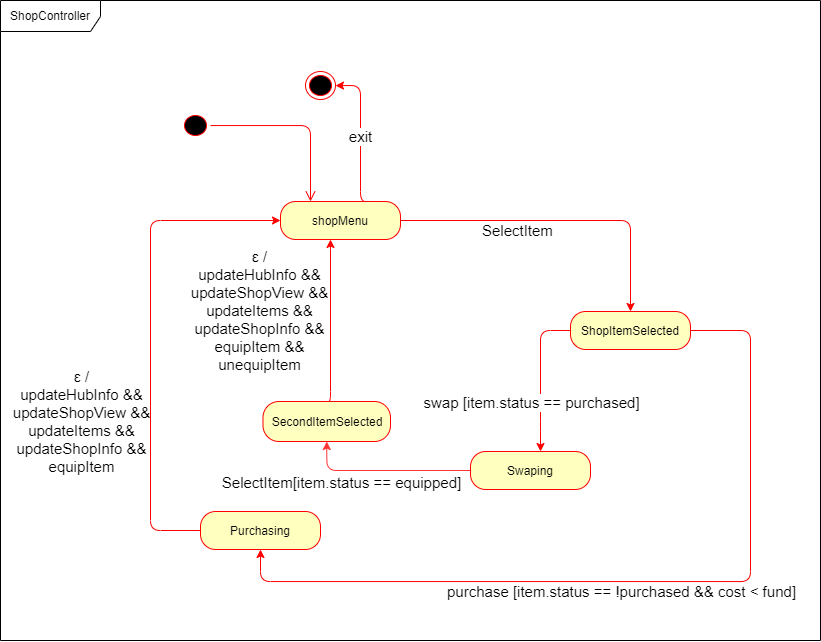
\includegraphics[width=\textwidth]{ShopController.png}
    \caption{State Diagram for Shop Controller Class.}
    \label{fig:ca}
\end{figure}
% End Section

\section{Sequence Diagrams}
\label{sec:sequence_diagrams}
%Begin Section
\begin{figure}[H]
    \centering
    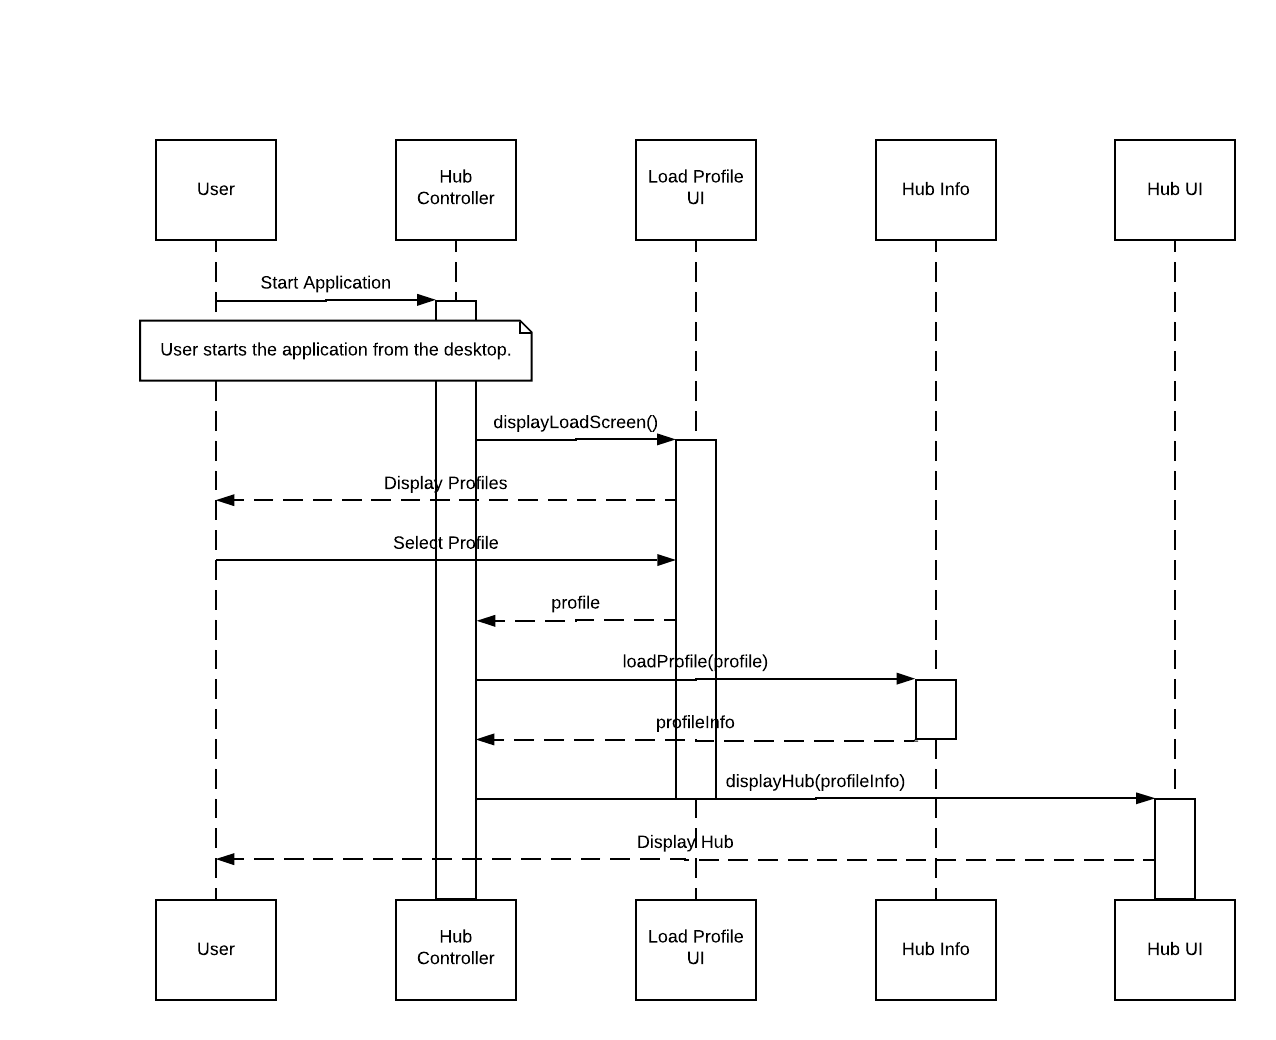
\includegraphics[width=\textwidth]{SD/LoadProfileSD.png}
    \caption{Sequence Diagram for the Load Profile use case.}
    \label{fig:sd}
\end{figure}

\begin{figure}[H]
    \centering
    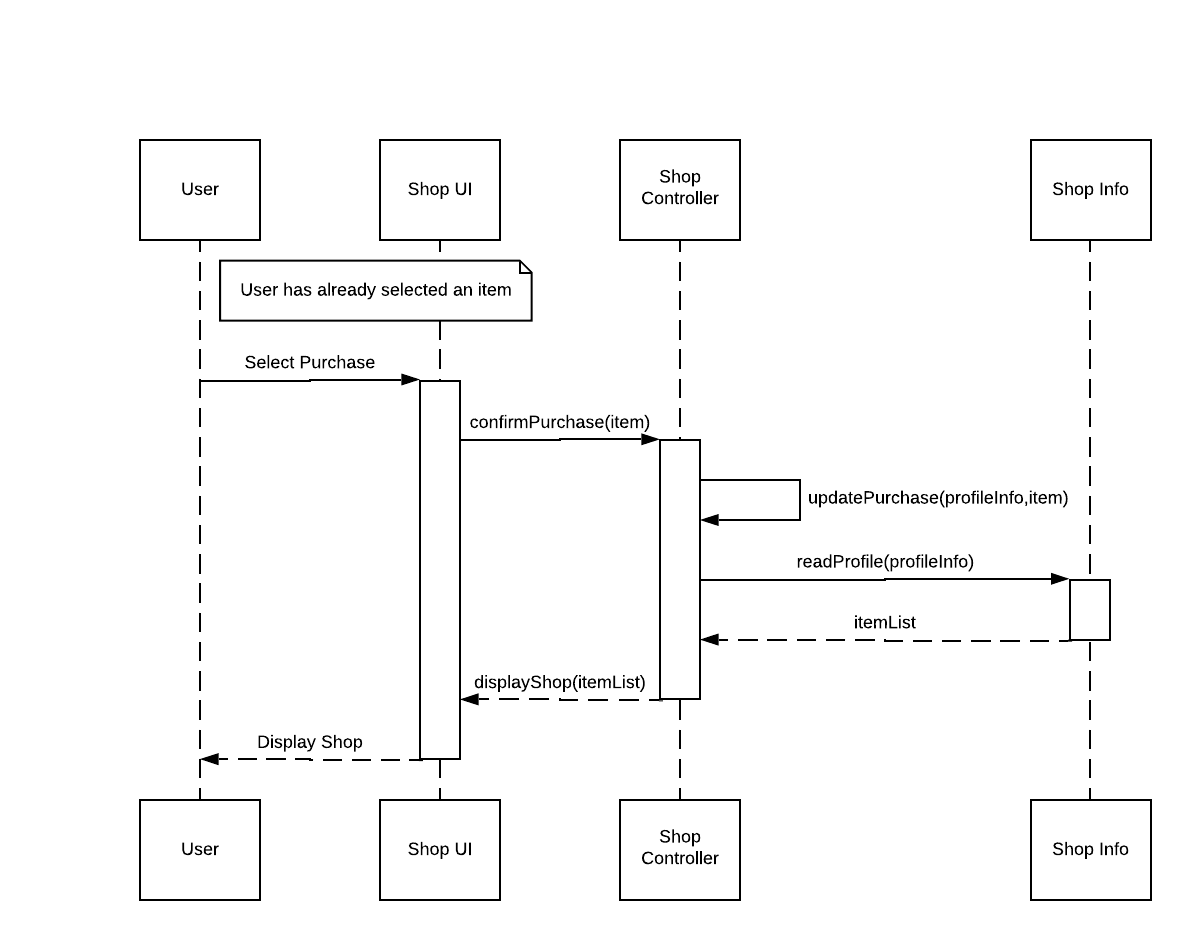
\includegraphics[width=\textwidth]{SD/PurchaseItemSD.png}
    \caption{Sequence Diagram for the Purchase Item use case.}
    \label{fig:sd}
\end{figure}

\begin{figure}[H]
    \centering
    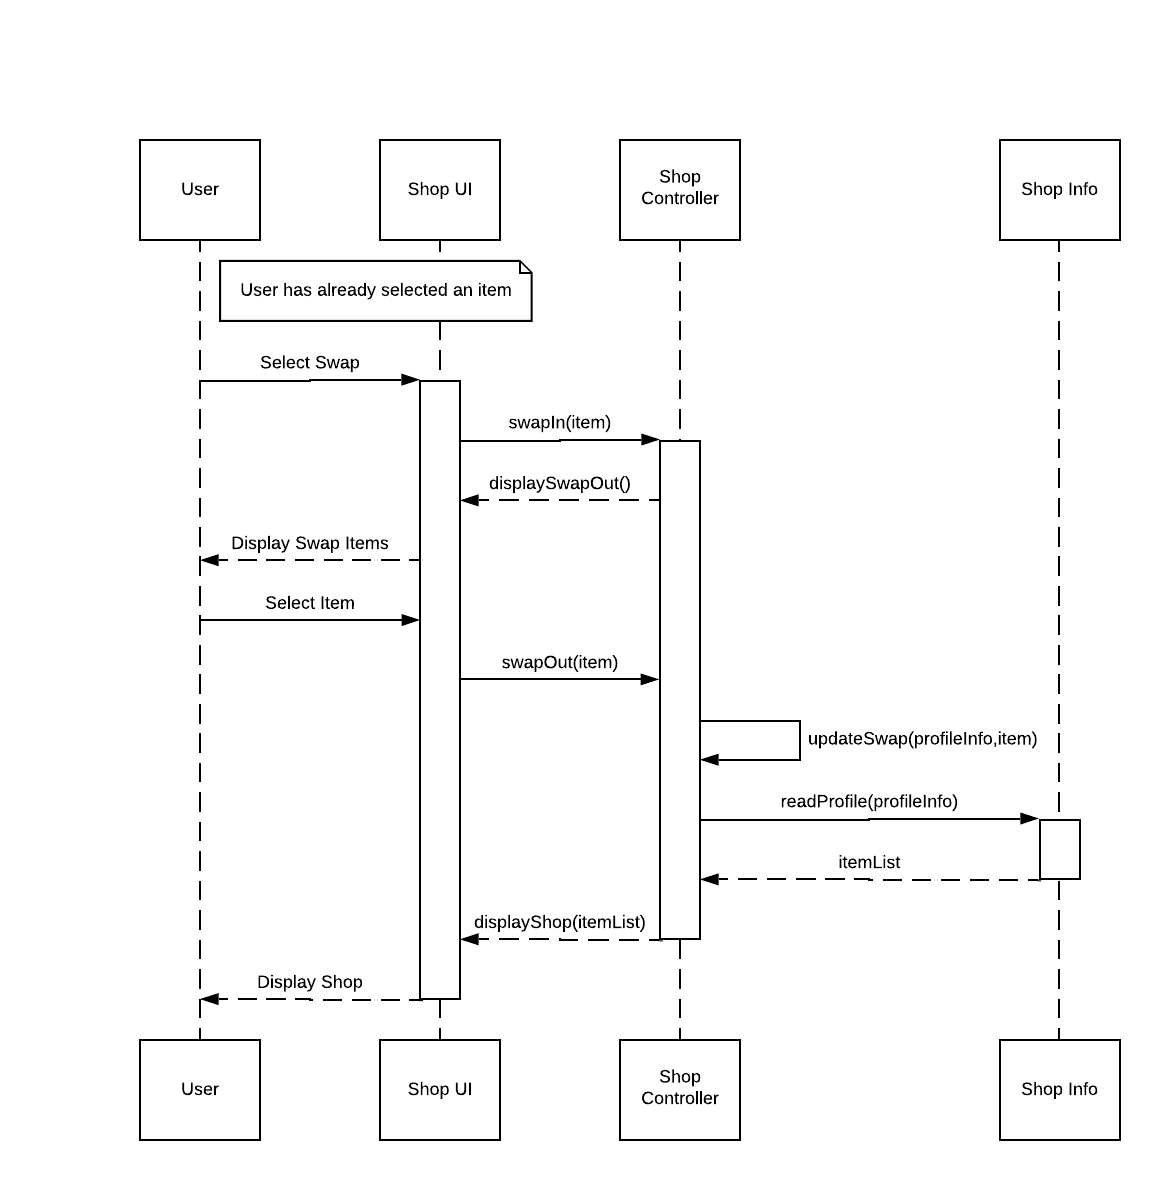
\includegraphics[width=\textwidth]{SD/SwapItemSD.png}
    \caption{Sequence Diagram for the Swap Item use case.}
    \label{fig:sd}
\end{figure}

\begin{figure}[H]
    \centering
    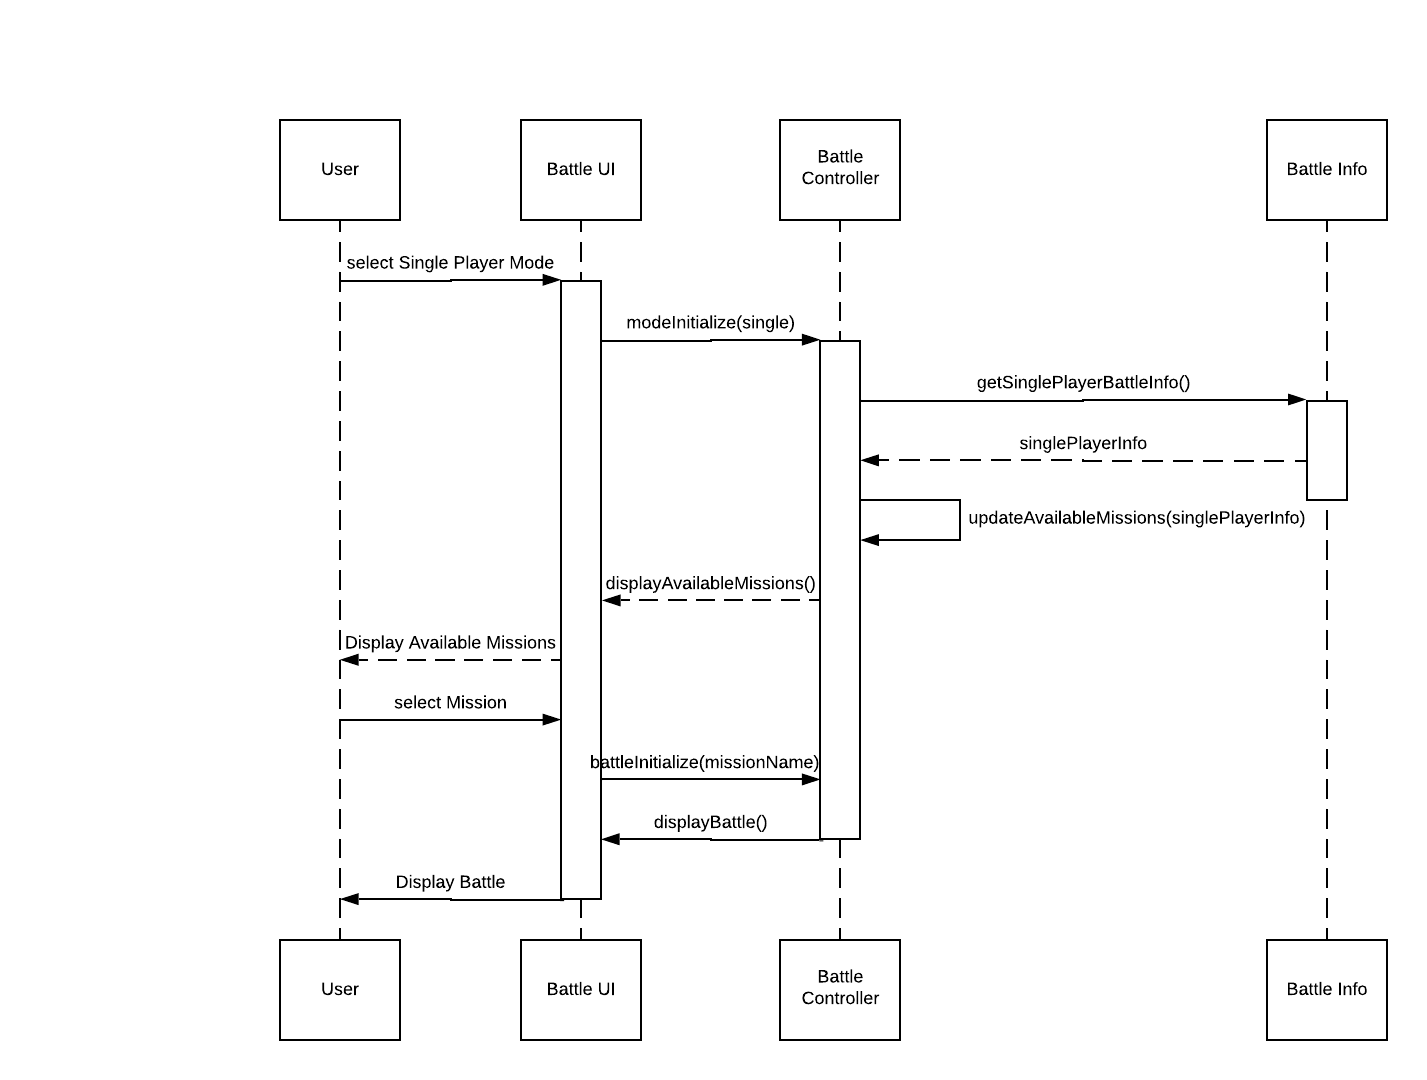
\includegraphics[width=\textwidth]{SD/EnterSinglePlayerBattle.png}
    \caption{Sequence Diagram for the Enter Single Player Battle use case.}
    \label{fig:sd}
\end{figure}

\begin{figure}[H]
    \centering
    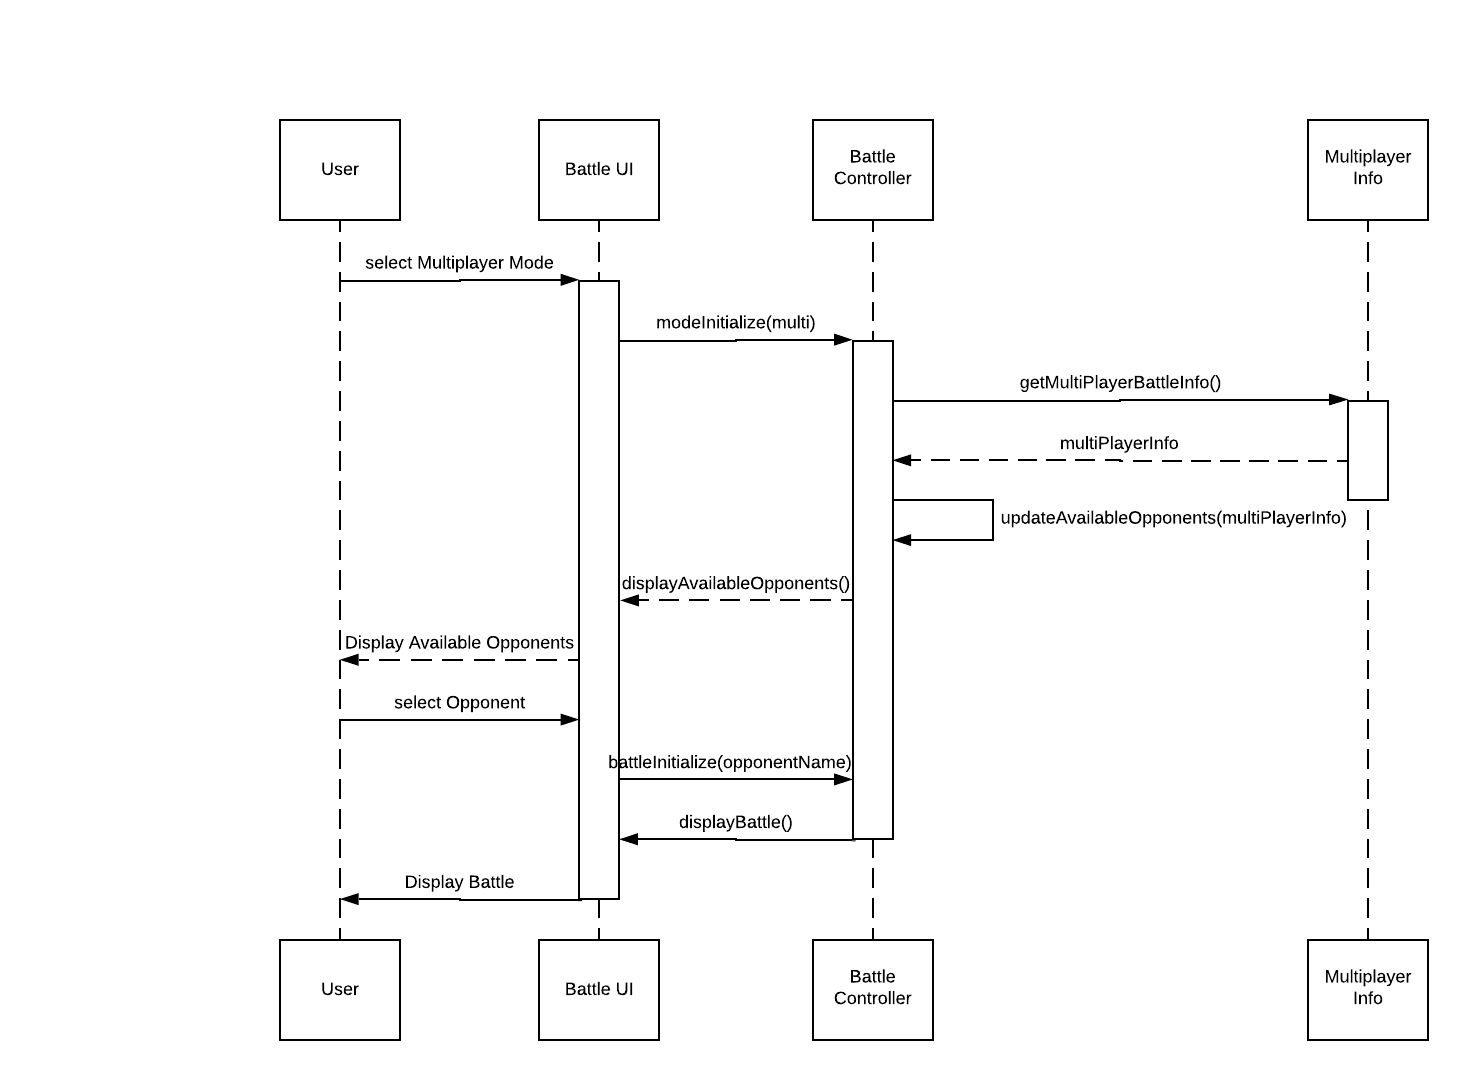
\includegraphics[width=\textwidth]{SD/EnterMultiplayerPlayerBattle.png}
    \caption{Sequence Diagram for the Enter Multiplayer Battle use case.}
    \label{fig:sd}
\end{figure}

\begin{figure}[H]
    \centering
    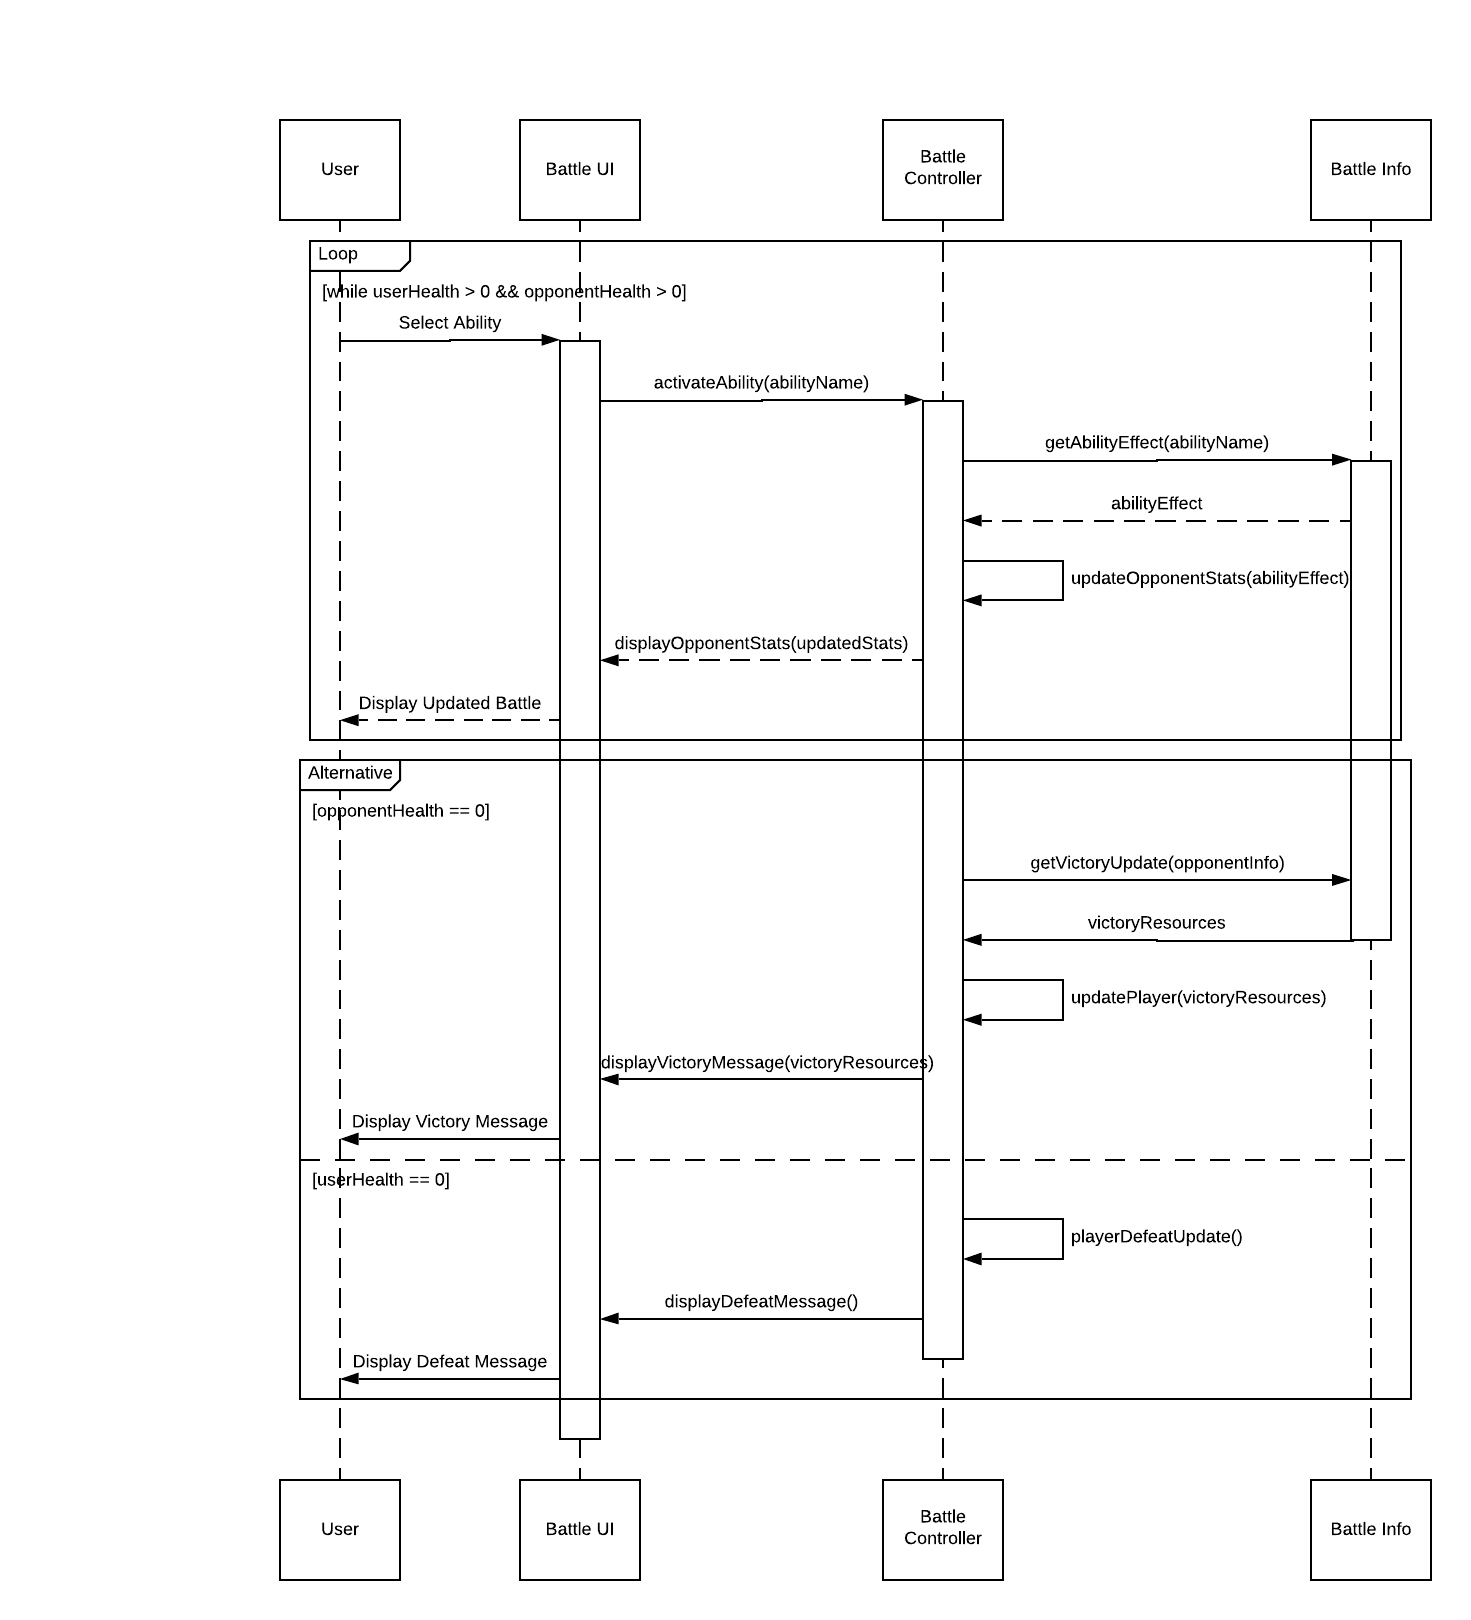
\includegraphics[width=\textwidth]{SD/SelectAbility.png}
    \caption{Sequence Diagram for the Select Ability use case.}
    \label{fig:sd}
\end{figure}


%End Section

\section{Detailed Class Diagram}
\label{sec:detailed_class_diagram}
% Begin Section
\begin{figure}[H]
    \centering
    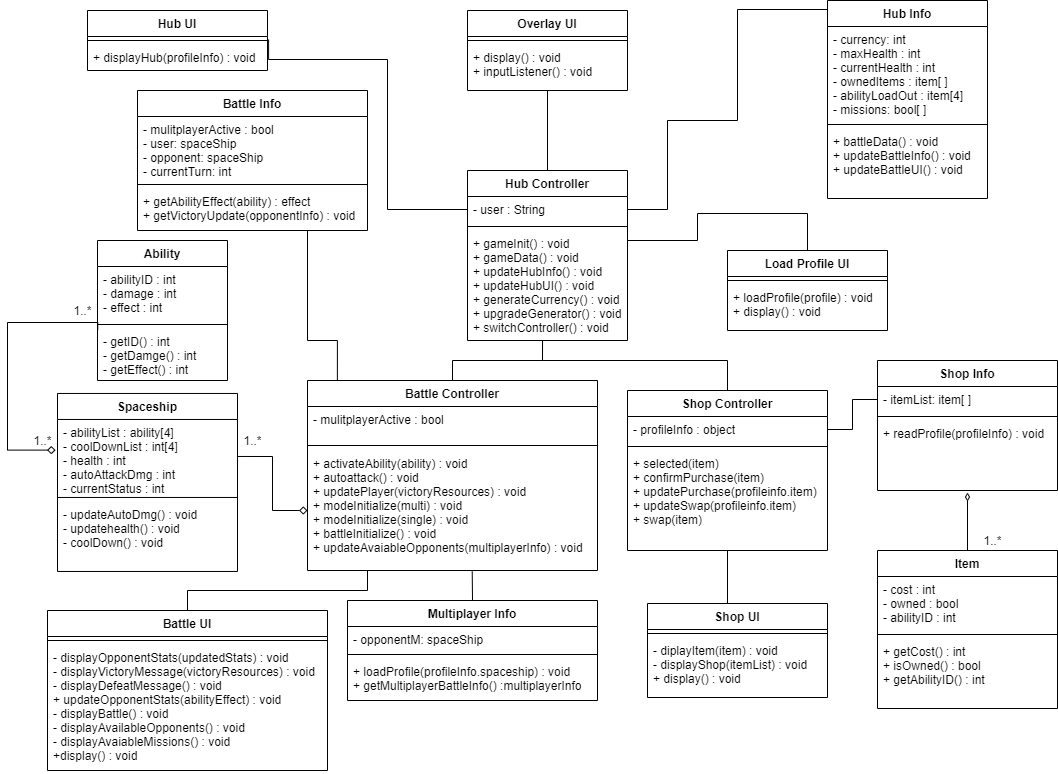
\includegraphics[width=\textwidth]{ClassDiagram.png}
    \caption{Class Diagram for the iSpaceship project.}
    \label{fig:ca}
\end{figure}
% End Section

\newpage
\appendix
\section{Division of Labour}
\label{sec:division_of_labour}
% Begin Section
Include a Division of Labour sheet which indicates the contributions of each team member. This sheet must be signed by all team members.
\\\\\\\\\\\\
\begin{tabular}{@{}p{.5in}p{4in}@{}}
Approved: & \hrulefill \\
& Group Member 1 \\\\\\\\\\
Approved: & \hrulefill \\
& Group Member 2 \\\\\\\\\\
Approved: & \hrulefill \\
& Group Member 3 \\\\\\\\\\
Approved: & \hrulefill \\
& Group Member 4 \\\\\\\\\\
Approved: & \hrulefill \\
& Group Member 5 \\\\\\\\\\
\end{tabular}
% End Section

\newpage
\section*{IMPORTANT NOTES}
\begin{itemize}
	\item You do \underline{NOT} need to provide a text explanation of each diagram; the diagram should speak for itself
	\item Please document any non-standard notations that you may have used
	\begin{itemize}
		\item \emph{Rule of Thumb}: if you feel there is any doubt surrounding the meaning of your notations, document them
	\end{itemize}
	\item Some diagrams may be difficult to fit into one page
	\begin{itemize}
		\item It is OK if the text is small but please ensure that it is readable when printed
		\item If you need to break a diagram onto multiple pages, please adopt a system of doing so and throughly explain how it can be reconnected from one page to the next; if you are unsure about this, please ask me
	\end{itemize}
	\item Please submit the latest version of Deliverable 1 and Deliverable 2 with Deliverable 3
	\begin{itemize}
		\item They do not have to be a freshly printed versions; the latest marked versions are OK
	\end{itemize}
	\item If you do \underline{NOT} have a Division of Labour sheet, your deliverable will \underline{NOT} be marked
\end{itemize}


\end{document}
%------------------------------------------------------------------------------